
\section{先行研究,方法}
ここでは、本研究で使用するCucumberの特徴について詳述します.
Cucumberはビヘイビア駆動開発(BDD)を実現するフレームワークです.
まずはbddの現れた背景や現状を示した後、Cucumberの記述の具体例を示して,
その特徴を詳述します.
さらに,本研究の対象となるmy\_helpの振る舞いを使用法とともに示します.

\subsection{RSpecとBDDについて}
ビヘイビア駆動開発(Behaviour-Driven Development : BDD)は,テスト駆動開発(Test-Driven Development : TDD)の工程への理解を深め,それをうまく説明しようとして始まりました.TDDの持つ単語のイメージが構造のテストを中心とするべしというのに対して,BDDはソフトの振る舞いに中心をおきなさいという意図があります.この違いが,初めに考えるべきテストの性質を変化させ,構造ではなく振る舞いを中心にテストを構築するという意識をもたせてくれます.

さらに,ソフトの中で,オブジェクト同士がコミュニケーションをとるように,実世界において開発チームやテストチーム,あるいはドキュメントチーム間のコミュニケーションの取り方をシステムで提供しようというのがBDDのフレームワークです.CucumberとRSpecはこれを実現する一つのシステムとして提供されています.

RSpecとCucumberの関係を図\ref{fig:001}に示しました.これは,The RSpec Book[1]から書き写した図です[1, pp.9].RSpecでテストを書くと一つ一つのfunctionあるいはmethodレベルでRed, Green, Refactoringを行うべしという意図があります.一方で,もっと大きな枠組み,つまりシステムレベルでもこれらのステップは必要です.ところが,それをRSpecで書くのには無理があります.このレベルのテスト記述をしやすくするのが,Cucumberです.そこでもRed, Green, Refactoringが必要で,そこでサイクルが回ることを意図しています.

\begin{figure}[htbp]\begin{center}
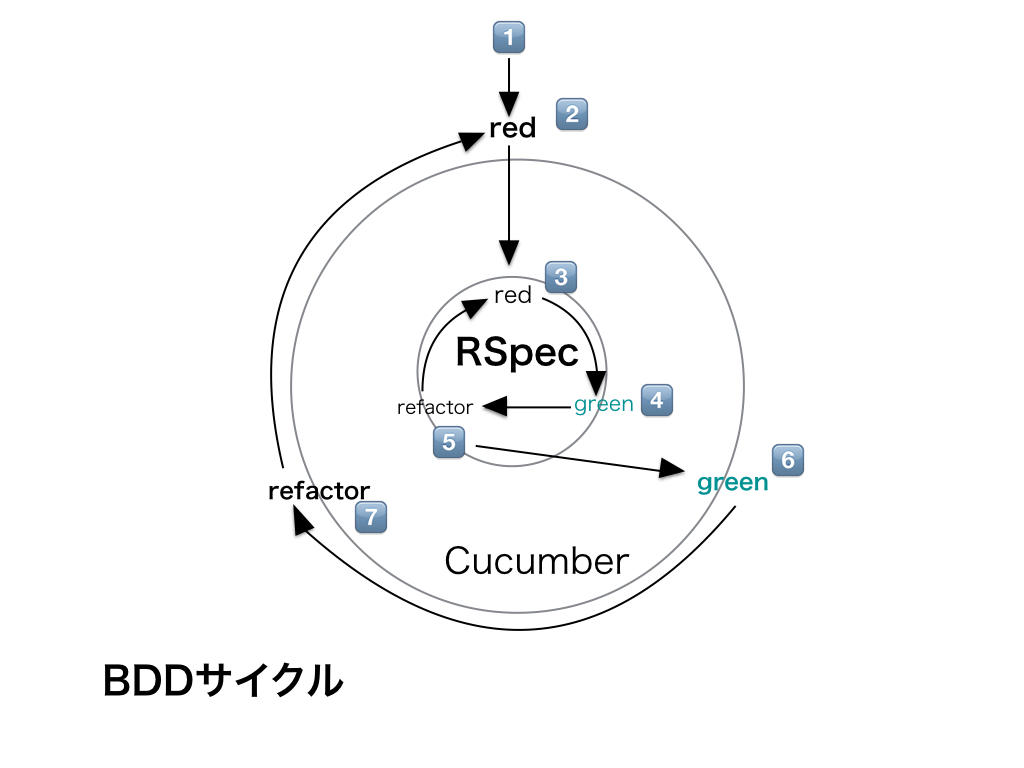
\includegraphics[width=12cm,bb= 0 0 937 753]{../figs/./my_help_nasu.001.jpeg}
\caption{RSpecとCucumberのRed-Green-Refactoringサイクル間の関係.}
\label{fig:001}
\label{default}\end{center}\end{figure}
BDDの基本的な考え方は次の通りまとめられています.

\begin{quotation}
BDDの目的は,ソフトウェアが使われる状況を説明するための言語を単純化することで,ソフトウェア開発チームのコミュニケーションを後押しすることです.つまり,あるコンテキストで(Given),あるイベントが発生すると(When),ある結果が期待されます(Then).BDDにおけるGiven, When, Thenの3つの単語は,アプリケーションやオブジェクトを,それらの振る舞いに関係なく表現するために使われる単純な単語です.ビジネスアナリスト,テスト担当者,開発者は皆,それらをすぐに理解します.これらの単語はCucumberの言語に直接埋め込まれています[1, pp.3-6].

\end{quotation}
手順を書き直すと図\ref{fig:002}の通りです.

\begin{figure}[htbp]\begin{center}
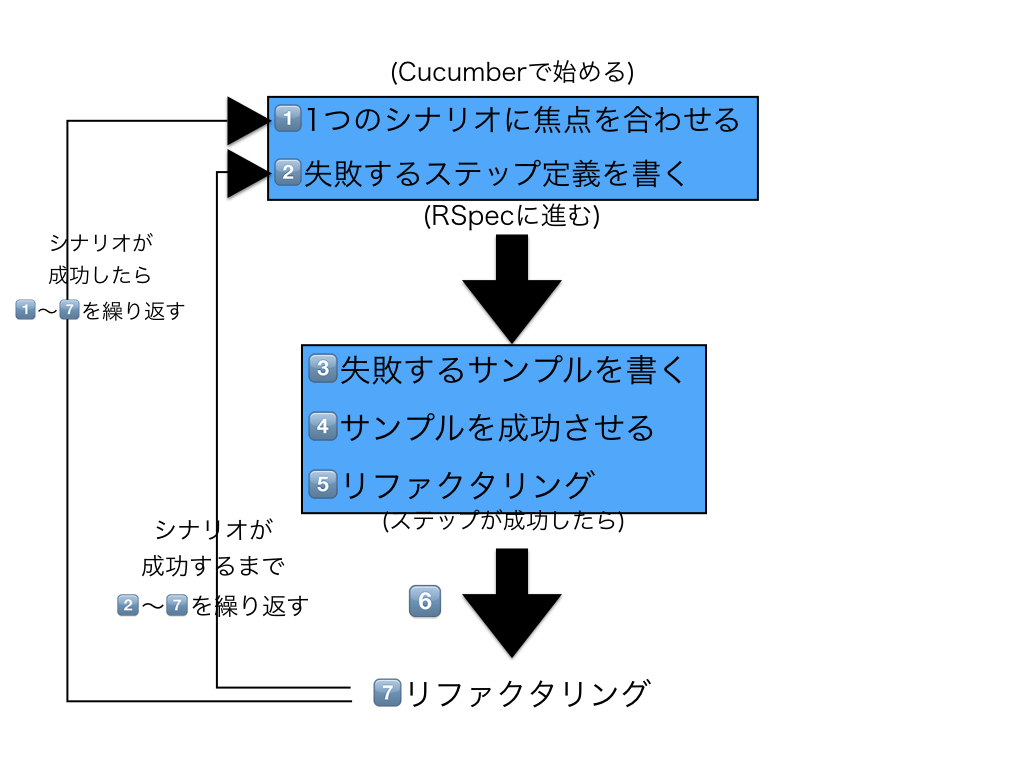
\includegraphics[width=12cm,bb= 0 0 937 753]{../figs/./my_help_nasu.002.jpeg}
\caption{RSpecとCucumberの手順.}
\label{fig:002}
\label{default}\end{center}\end{figure}
まずCucumberで一つのシナリオに焦点を当てて,その振る舞いを記述するfeatureを書きます.一つずつつぶしていくのがこつです.一つのfeatureが書けたら、次に,それぞれfeatureを実現するステップに分けて仕様を決めて行きます.これはTDDのred green refactoringの前に行う作業,「仕様を決める」に対応しています.このプロセスが終了したら,RSpecに行きます.
RSpecでは実際にテストコードを書き,ここでもred, green, refactoringを行います.
RSpecが成功したら,Cucumberのrefactoringを行います.

